% ----------------------------------------------
%
%	Damian Skrzypiec
% 	20.04.2017
%	Draft of Master Thesis - Mathematics
%
% ----------------------------------------------

\documentclass{pracamgr}



\usepackage[UTF8]{inputenc}
\usepackage{latexsym}
\usepackage{amsmath}
\usepackage{amsthm}
\usepackage{amssymb}
\usepackage{algorithm}
\usepackage{algpseudocode}


% ----------------------
% For Geogebra
% ----------------------

\usepackage{pgf,tikz}
\usetikzlibrary{shapes.geometric}
\usepackage{color}
\usetikzlibrary{arrows}
\usepackage{xcolor}
%\usepackage[latin2]{inputenc}
%\usepackage[utf8]{inputenc}
\usepackage{latexsym}
\usepackage{graphicx,wrapfig,lipsum}

\definecolor{qqqqff}{rgb}{0.,0.,1.}

% Symbol for conditional independence
\newcommand*{\bigCI}{%
  \mathrel{\text{%
    {\rotatebox[origin=c]{90}{\resizebox{2.25ex}{1.65ex}{$\vDash$}}}%
  }}%
}

\theoremstyle{definition}

% Propositions 
\newtheorem{prop}{Proposition}[section]
\newtheorem{thm}{Theorem}[section]
\newtheorem{ex}{Example}[section]
\newtheorem{remark}{Remark}[section]

% Definition of symbol C-Separation
\newcommand{\cSep}[4]{\ensuremath{\left\langle #1 , #2 \mid #3 \right\rangle_{\mathcal{#4}}^{sep}}}

% Short for \mathcal{}
\newcommand{\mc}[1]{\ensuremath{\mathcal{#1}}}
\newcommand{\mb}[1]{\ensuremath{\mathbb{#1}}}


% Dane magistranta:

\author{Damian Skrzypiec}

\nralbumu{320335}

\title{Structure Learning Algorithms for Chain Graphs}

\tytulang{Algorytmy uczenia strukturalnego dla grafów łańcuchowych}

%kierunek: Matematyka, Informatyka, ...
\kierunek{Mathematics}


% Praca wykonana pod kierunkiem:
% (podać tytuł/stopień imię i nazwisko opiekuna
% Instytut
% ew. Wydział ew. Uczelnia (jeżeli nie MIM UW))
\opiekun{John Noble, PhD.\\
  Institute of Applied Mathematics and Mechanics\\
  }

% miesiąc i~rok:
\date{April 2017}

%Podać dziedzinę wg klasyfikacji Socrates-Erasmus:
\dziedzina{ 
11.2 Statistics\\ 
}

%Klasyfikacja tematyczna wedlug AMS (matematyka) lub ACM (informatyka)
\klasyfikacja{62 Statistics \\
		62C10 Bayesian Problems \\
		}

% Słowa kluczowe:
\keywords{graphical model, chain graph, structure learning}

% Tu jest dobre miejsce na Twoje własne makra i~środowiska:
\newtheorem{defi}{Definition}[section]

% koniec definicji

\begin{document}
\maketitle

\begin{abstract}
  In this place will be abstract of this project.
\end{abstract}

\tableofcontents
\listoffigures
\listofalgorithms
\addtocontents{loa}{\def\string\figurename{Algorithm}}
%\listoftables

\chapter{Introduction}

% ---------------------------------------
%	Damian Skrzypiec
%	IV 2017
%	Introduction
% ---------------------------------------


The purpose of this project is to present algorithms for learning conditional independence structure of joint probability distributions represented by chain graphs. This is a special case of learning probabilistic graphical models which provides convenient representation of factorisation probability distribution using graphs.
Well-known and well-examined examples of probabilistic graphical models (PGMs) are Bayesian Networks where PGM is represented by directed acyclic graph and Markov Fields where PGM is represented by undirected graph. Chain graphs is a class of graphs that does not contains cycles (formal definition in \ref{chainGraphDef}). It contains both directed acyclic graphs and undirected graphs hence it is natural generalization of Bayesian Networks and Markov Fields.
In this paper we present one algorithm for learning chain graphs and one algorithm for learning undirected graphical models. Both algorithms are based on idea of graph decomposition which suppose to decrease complexity of algorithms.


\chapter{Preliminaries}\label{r:prelim}

	\section{Graph Theory Terminology}\label{r:defGraph}
		% ----------------------------------------------
%
%	Damian Skrzypiec
% 	03.05.2017
%	Graph Theory Definitions
%
% ----------------------------------------------


This section provides definitions of graph theory objects required for completeness of further sections.
In this section, when is not mention different, $V$ is default notation for set of graph's vertices and 
$E$ is default notation for set of graph's edges. 


% ----------------------
% Undirected edge
% ----------------------
\begin{defi}{\textbf{(Undirected edge)}} \\
	For vertices $u, v \in V$ we say that there is an undirected edge between vertices $u$ 
	and $v$ if $(u, v) \in E$ and $(v, u) \in E$. Undirected edge between $u$ and $v$ is marked as $u-v$.
\end{defi}


% ----------------------
% Directed edge
% ----------------------
\begin{defi} {\textbf{(Directed edge)}} \\
	For vertices $u, v \in V$ we say that there is a directed edge from vertex $u$ to vertex $v$ if
	$(u, v) \in E$ and $(v, u) \notin E$. Directed edge from $u$ to $v$ is marked as $u \rightarrow v$.
\end{defi}


% ----------------------
% Sekelton
% ----------------------
\begin{defi} {\textbf{(Skeleton)}} \\
	Skeleton of graph $G = (V, E)$ is a graph $G' = (V', E')$ where $V = V'$ and the set of edges $E'$
	is obtained by replacing directed edges of set $E$ by undirected edges.
\end{defi}


% ----------------------
% Route
% ----------------------
\begin{defi} {\textbf{(Route)}} \\
	A \textit{route} in graph $G = (V, E)$ is a sequence of vertices $(v_0, \dots, v_k)$, $k \ge 0$, such that 
	$$ (v_{i-1}, v_i) \in E \ \  \mbox{or} \ \ (v_i, v_{i-1}) \in E$$
	for $i = 1, \dots, k$. The vertices $v_0$ and $v_k$ are called \textit{terminals}. A route is called descending
	if $(v_{i-1}, v_i) \in E$ for $i = 1, \dots, k$. Descending route from $u$ to $v$ is marked as $u \mapsto v$. 
\end{defi}


% ----------------------
% Path
% ----------------------
\begin{defi} {\textbf{(Path)}} \\
	A route $r = (v_0, v_1, \dots, v_k)$ in graph $G = (V, E)$ is called a path if all vertices in $r$ are distinct.
\end{defi}


% ----------------------
% Complex
% ----------------------
\begin{defi} \label{complexDef} {\textbf{(Complex)}} \\
	A path $\pi = (v_1, v_2, \dots, v_k)$ in graph $G = (V, E)$ is called complex if
	\begin{enumerate}
		\item $v_1 \rightarrow v_2$
		\item $\forall_{i \in \left\{ 2, 3, \dots k-2 \right\}} \ v_i - v_{i+1}$
		\item $v_{k-1} \leftarrow v_k$
		\item There is not additional edges in graph $G$ for vertices in path $\pi$.
	\end{enumerate}
	Vertices $v_1$ and $v_k$ are called \textit{parents} of the complex, set of vertices 
	$\left\{v_2, v_3, \dots, v_{k-1} \right\}$ is called \textit{region} of the complex and number
	$k-2$ is the \textit{degree} of the complex.
\end{defi}
Next we define extended version of moral graphs. In Bayesian Networks moral graph is 
an undirected graph obtained from the original graph by adding undirected edges for not connected parents of the same child and then transform all edges into undirected edges. In case of chain graphs there can be situation when there are 
not connected parents of connected children (see \ref{fig:ImmoralCG}). 
This situation can be interpreted as immoral and to be moralized a connection between parents are required.


\begin{ex} {\textbf{(Immorality in chain graph)}}
	\begin{figure}[h]
		\centering
		\vspace{-10pt}
		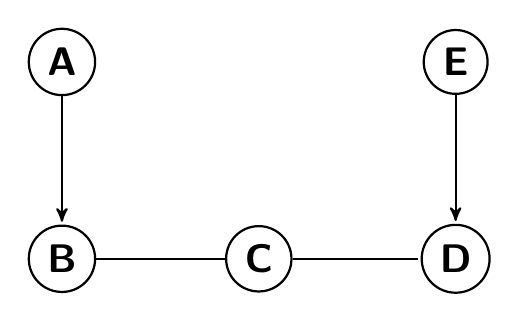
\begin{tikzpicture}[>=stealth',shorten >=1pt,auto,node distance=2.5cm,
		                    thick,main node/.style={circle,draw,font=\sffamily\Large\bfseries}]
			% Nodes
			  \node[main node] (A) {A};
			  \node[main node] (B) [below of = A] {B};
			  \node[main node] (C) [right of = B] {C};
			  \node[main node] (D) [right of = C] {D};
			  \node[main node] (E) [above of = D] {E};
			
			% Edges
			  \draw[->] (A) -- (B);
			  \draw     (B) -- (C) -- (D);
			  \draw[->] (E) -- (D);
			\end{tikzpicture}
			
		\caption{Immorality in chain graph}			
		\label{fig:ImmoralCG} 
	\end{figure}
\end{ex}

% ----------------------
% Moral Graph
% ----------------------
\begin{defi} \label{moralGraphDef} {\textbf{(Moral Graph)}} \\
	Let $G = (V, E)$ be a graph. A moral graph $G^{m} = (V, E^{m})$ of graph $G$ is a graph obtained by firstly join parents of complexes in graph $G$ and then replace all edges by undirected edges.
\end{defi}


% ----------------------
% Cycles
% ----------------------
\begin{defi} {\textbf{(Cycle)}} \\
	A route $r = (v_0, v_1, \dots, v_k)$ in graph $G = (V, E)$ is called a pseudocycle if $v_0 = v_k$ and 
	a cycles if further route is a path and $k \ge 3$.
\end{defi}

A graph with only directed edges is called an \textit{undirected graph}. A graph without directed cycles 
and with only directed edges is called a \textit{directed acyclic graph} (DAG).


% ----------------------
% Chain graph
% ----------------------
\begin{defi}\label{chainGraphDef} {\textbf{(Chain graph)}}  \\
	A graph $G = (V, E)$ is called a chain graph if it does not have directed (pseudo) cycles.
\end{defi}



% ----------------------
% Section
% ----------------------
\begin{defi} {\textbf{(Section)}} \\
	A subroute $\sigma = (v_i, \dots, v_j)$ of route $\rho = (v_0, \dots, v_k)$ in graph $G$ is called section if $			\sigma$ is the maximal undirected subroute of route $\rho$. That means $v_i - \dots - v_j$ for $0 \le i \le j 			\le k$. Vertices $v_i$ and $v_j$ are called terminals of section $\sigma$. Further vertex $v_i$ is called a 			head-terminal if $i>0$ and $v_{i-1} \rightarrow v_i$ in graph $G$. Analogically vertex $v_j$ is called 
	a head-terminal if $j<k$ and $v_j \leftarrow v_{j+1}$ in graph $G$.
\end{defi}


A section with two head-terminals is called \textit{head-to-head} section. Otherwise the section is called 
\textit{non head-to-head}. For a given set of vertices $S \subset V$ in graph $G$ and section $\sigma = (v_i, \dots, v_j)$ we say that section is hit by $S$ if $\left\lbrace v_i , \dots, v_j \right\rbrace \cap S \neq \emptyset$. Otherwise we say that section $\sigma$ is outside set $S$.



% ----------------------
% Intervention
% ----------------------
\begin{defi} {\textbf{(Intervention)}} \\
	A route $\rho$ in graph $G = (V, E)$ is blocked by a subset $S \subset V$ of vertices if and only if there 				exists a section $\sigma$ of route $\rho$ such that one of the following conditions is satisfied.
	
	\begin{enumerate}
		\item Section $\sigma$ is head-to-head with respect to $\rho$ and $\sigma$ is outside of $S$.
		\item Section $\sigma$ is non head-to-head with respect to $\rho$ and $\sigma$ is hit by $S$.
	\end{enumerate}
	
\end{defi}



\begin{ex} {\textbf{(Graph definitions)}} \\
	Based on the following two graphs (figures \ref{fig:ExampleGraph} and \ref{fig:ExampleMoralGraph}) we 
	present examples of above defined definitions. Let graph 
	presented in figure \ref{fig:ExampleGraph} be denoted as $G$. In graph $G$ as example of descending 
	route is $(A, B, C, D)$ and 
	example of non-descending route is $(D, E, F, G)$. Graph $G$ contains two complexes. Complex $(A, B, C, D, E)$
	is of degree equal to $3$ and the other one $(F, G, H, I)$ is of degree equal to $2$. Graph $G$ contains one cycle
	$(I, J, K, I)$. The Route $(F, G, H, I)$ in graph $G$ contains section $(G, H)$ which is head-to-head section.

	\begin{figure}[h]
		\centering
		\vspace{-10pt}
		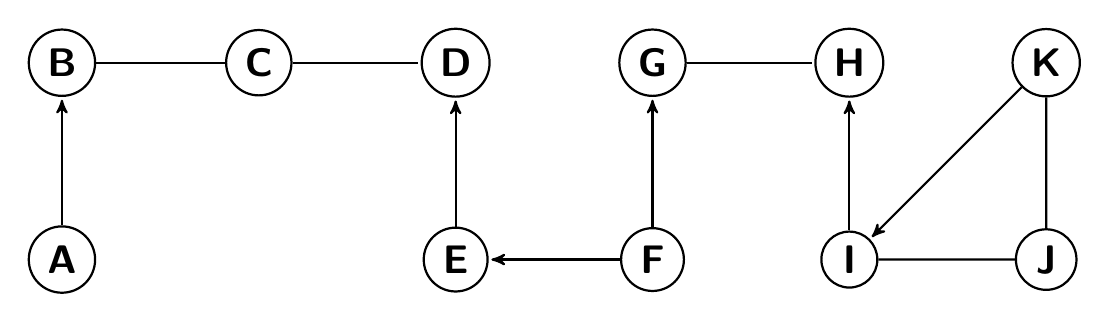
\begin{tikzpicture}[>=stealth',shorten >=1pt,auto,node distance=2.5cm,
		                    thick,main node/.style={circle,draw,font=\sffamily\Large\bfseries}]
			% Nodes
			  \node[main node] (A) {A};
			  \node[main node] (B) [above of = A] {B};
			  \node[main node] (C) [right of = B] {C};
			  \node[main node] (D) [right of = C] {D};
			  \node[main node] (E) [below of = D] {E};
			  \node[main node] (F) [right of = E] {F};
			  \node[main node] (G) [above of = F] {G};
			  \node[main node] (H) [right of = G] {H};
			  \node[main node] (I) [below of = H] {I};
			  \node[main node] (J) [right of = I] {J};
			  \node[main node] (K) [above of = J] {K};
			
			% Edges
			  \draw[->] (A) -- (B);
			  \draw     (B) -- (C) -- (D);
			  \draw[->] (E) -- (D);
			  \draw[->] (F) -- (E);
			  \draw[->] (F) -- (G);
			  \draw     (G) -- (H);
			  \draw[->] (I) -- (H);
			  \draw[->] (I) -- (J) -- (K) -- (I);
			\end{tikzpicture}
			
		\caption{Example graph}			
		\label{fig:ExampleGraph} 
	\end{figure}
	
	Graph presented in figure \ref{fig:ExampleMoralGraph} is moral graph of graph $G$. 
	Additional undirected edges $A - E$ and $F - I$ are the result of connecting parents of complexes in 
	the original graph $G$.
	
	\begin{figure}
	 	\centering
	 	\vspace{-10pt}
	 	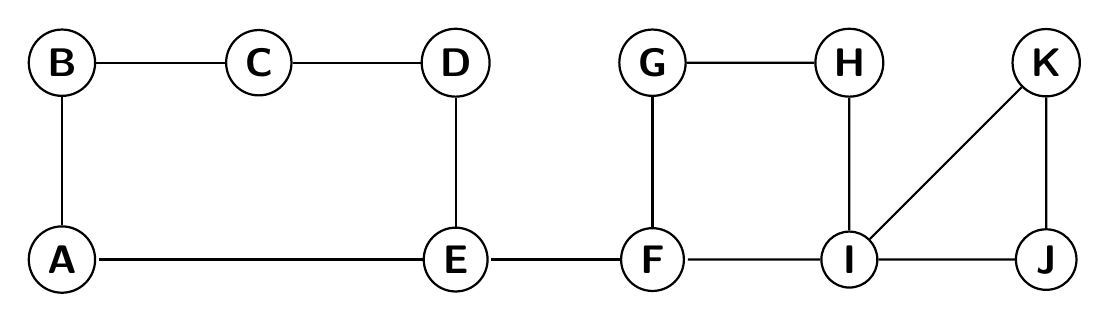
\begin{tikzpicture}[>=stealth',shorten >=1pt,auto,node distance=2.5cm,
		                    thick,main node/.style={circle,draw,font=\sffamily\Large\bfseries}]
			% Nodes
			  \node[main node] (A) {A};
			  \node[main node] (B) [above of = A] {B};
			  \node[main node] (C) [right of = B] {C};
			  \node[main node] (D) [right of = C] {D};
			  \node[main node] (E) [below of = D] {E};
			  \node[main node] (F) [right of = E] {F};
			  \node[main node] (G) [above of = F] {G};
			  \node[main node] (H) [right of = G] {H};
			  \node[main node] (I) [below of = H] {I};
			  \node[main node] (J) [right of = I] {J};
			  \node[main node] (K) [above of = J] {K};
			
			% Edges
			 \draw (A) -- (B) -- (C) -- (D) -- (E) -- (A);
			 \draw (G) -- (F) -- (E);
			 \draw (F) -- (G) -- (H) -- (I) -- (J) -- (K) -- (I) -- (F);
			\end{tikzpicture}
			
		\caption{Moral graph of graph in figure \ref{fig:ExampleGraph}}			
		\label{fig:ExampleMoralGraph} 
    \end{figure}		
	
	
\end{ex}




		
	\section{Graphical Model Terminology}\label{r:defGraphModel}
		
% ----------------------
% Conditional independence
% ----------------------
%
Our main goal is to find an conditional independence structure of given joint probability distribution, hence we start from recalling definition of conditional independence.

\begin{defi} \label{condInd} (Conditional Independence) \\
	Let $(X_1, X_2, \dots, X_n)$ be a random vector over probability space $(\Omega, \mathcal{F}, \mathbb{P})$.
	We say that random vectors $X_A = \left\{ X_a  \ | \ a \in A \right\}$ and 
	$X_B = \left\{ X_b  \ | \ b \in B \right\}$
	are conditional independent given $X_S = \left\{ X_s  \ | \ s \in S \right\}$ when 
	for all $A_1, A_2, A_3 \in \mathcal{F}$
	%
	\begin{equation} 
		\mathbb{P}(X_A \in A_1, X_B \in A_2 \mid X_S \in A_3) = \mathbb{P}(X_A \in A_1 \mid X_S \in A_3) 													\mathbb{P}(X_B \in A_2 \mid X_S \in A_3)
	\end{equation}
	%
	where $A, B, S \subset {1, 2, \dots, n}$. Conditional independence of $X_A$ and $X_B$
	given $X_S$ is denoted as $X_A \bigCI X_B \mid X_S$.
\end{defi}
The following definition of c-separation is an analogical version of d-separation, used in Bayesian Networks, for chain graphs. This definition was introduced by Studeny and Bouckaert in \cite{OCG}. The notation c-separation is short of "chain separation" and it is written in this form to present analogy to definition of d-separation.


% ----------------------
% c-separation
% ----------------------
\begin{defi} \label{cSepDef} (c-separation) \\
	Let $G = (V, E)$ be a chain graph. Let $A, B, S$ be three disjoint subsets of the vertex set $V$, such that
	$A$ and $B$ are nonempty. We say that $A$ and $B$ are c-separated by $S$ on $G$ if every route within one of 
	its terminals in $A$ and the other in $B$ is blocked by $S$. 
	We call $S$ a c-separator for $A$ and $B$ and mark as \cSep{A}{B}{S}{G}.
\end{defi}


% ----------------------
% Faithfulness and Markovian
% ----------------------
\begin{defi} \label{faithDef} (faithfulness) \\
	Let $G = (V, E)$ be a chain graph with random variables $X_v$ associated with vertex $v \in V$. Let note domain of 
	random variable $X_v$ as $\mathcal{X}_v$. A probability measure $\mathbb{P}$ 
	defined on $\prod_{v \in V} \mathcal{X}_v$ is \textit{faithful} with respect to $G$ if 
	for any triple $(A, B, S)$ of disjoint subsets of $V$ where $A$ and $B$ are non-empty we have
	%
	\begin{equation}
		\cSep{A}{B}{S}{G} \iff X_A \bigCI X_B \mid X_S
	\end{equation}
	%	
	In the same setup a probability measure $\mathbb{P}$ is called \textit{Markovian} with respect to $G$ if
	%
	\begin{equation}
		\cSep{A}{B}{S}{G} \Longrightarrow X_A \bigCI X_B \mid X_S
	\end{equation}
	%
\end{defi}
The following theorem from Frydenberg's paper \cite{CGMP} provides convenient tool for testing if two given 
chain graphs are the same in respect to Markov equivalent class.

% ----------------------
% Markov equivalence of chain graphs
% ----------------------
\begin{prop} (Markov equivalence of chain graphs) [Theorem 5.6 from \cite{CGMP}] \\
	Two chain graphs $G_1 = (V_1, E_1)$ and $G_2 = (V_2, E_2)$ have the same Markov properties if and only if they same 
	the same skeleton and the same complexes.
\end{prop}	






\chapter{LCD Algorithm} \label{chap:LCDAlg}

	% ----------------------------------------------
%
%	Damian Skrzypiec
% 	August 2017
%	LCD Algorithm overview.
%
% ----------------------------------------------

LCD algorithm is short for \textit{Learning of Chain graphs via Decomposition} algorithm. The algorithm was introduced by Ma, Xie and Geng in paper 
\textit{Structural Learning of Chain Graphs via Decomposition} \cite{CG}. LCD algorithm returns 
representative chain graph of it's Markov equivalence class, because even with perfect knowledge of data probability
distribution any two chain graph structures within the same Markov equivalence class are indistinguishable. 
The algorithm is composed of two steps - recovering skeleton of chain graph and the second is recovering complexes. This
idea is backed up by proposition \ref{markovEquivThm}. 
The main idea of skeleton recovery is to decompose set of variables into smaller sets, determine independence structure there and join results in a correct way. 
To decompose problem into smaller subproblems concept of separation trees is being used.
The LCD algorithm required assumption about faithfulness of a probability distribution to some chain graph. This assumption is not very restrictive, because Jose Pena proved that the
set of strictly positive probability distributions that are not faithful to some chain graph G has zero Lebesgue measure. Pena proved it for dicrete case in $2009$ in \cite{FaithDicr}
(theorem $5$) and later in $2011$ for gaussian case in \cite{FaithGauss} (theorem $4.2$).




	\section{Decomposition of chain graphs}
		
		\subsection{Separation Trees}
			% ----------------------------------------------
%
%	Damian Skrzypiec
% 	August 2017
%	LCD Algorithm - section about separation trees.
%
% ----------------------------------------------

\tikzset{
    triangle/.style={
        draw,regular polygon,
        regular polygon sides=3,
        minimum size = 1pt,
        text width = 1cm,
        inner sep = 0pt,
        align = center
    }
}

\tikzstyle{block} = [draw, rectangle, minimum width = 0.75cm, minimum height = 0.75cm]



\begin{defi} {\textbf{(Node Tree)}} \\ 
	Let $G = (V, E)$ be a graph and $\mathcal{C} = \left\{ C_1, \dots, C_k\right\}$ be a collection of distinct 
	vertices sets such that $\forall i \in \left\{1, 2, \dots, k \right\} C_i \subset V$. 
	A node tree is a graph which set of vertices are equal to $\mathcal{C}$ and it contains undirected edges between
	every nodes $C_i$ and $C_j$. Moreover for every edge $e$ between $C_i$ and $C_j$ we add separator 
	$S(C_i, C_j) = C_i \cap C_j$ into set of nodes. Nodes $C_i$ are displayed by triangle and separators are
	displayed by rectangles. Notation for node tree is $\mathcal{T}(G, \mathcal{C})$.
\end{defi}


\textbf{TODO: Example of Node tree}

\begin{defi} {\textbf{(Splitting Node Tree by separator)}} \\ 
	Some definition.
\end{defi}


\begin{defi} {\textbf{(Separation tree)}} \\
	For given chain graph $G = (V, E)$ and node set $\mathcal{C}$ we say that node tree $\mathcal{T}(G, \mathcal{C})$
	is a separation tree if 

	\begin{enumerate}
		\item $\cup_{C \in \mathcal{C}} C = V$ and
		\item for any separator $S = S(C_i, C_j)$ in node tree $\mathcal{T}(G, \mathcal{C})$ with $V_1$ 
		and $V_2$ as subtrees obtained by removing separator $S$ we have  
		$$ \cSep{V_1 \setminus S}{V_2 \setminus S}{S}{G} $$
	\end{enumerate}		
	
\end{defi}


\begin{figure}[h]
	\centering
	\vspace{-10pt}
	\begin{tikzpicture}[>=stealth',shorten >=1pt,auto,node distance=2.5cm,
	                    thick,main node/.style={circle,draw,font=\sffamily\Large\bfseries}]
	                    
		% Nodes
		 \node[block, name = A] {A};
		 \node[block, right of = A] (B) {B};
		 \node[triangle, right of = B] (C) {C D H O};
		 \node[block, right of = C] (D) {E, F, G};
		 
		 \draw[->] (A) -- (B);
		 \draw 		(B) -- (C);
		 \draw[->] (C) -- (D);

	\end{tikzpicture}
		
	\caption{Separation Tree}			
\end{figure}
			
		\subsection{Construction of Separation Trees}
			% ----------------------------------------------
%
%	Damian Skrzypiec
% 	August 2017
%	Constructing separation trees.
%
% ----------------------------------------------


In this subsection we present method for construction a separation trees by using labeled block ordering.
Concept of labeled block ordering was introduced by Roverto and La Rocca in \cite{LBO}.  
\textbf{TODO:} extend description  


\begin{defi} (labelled block ordering) \\ 
	Let $G = (V, E)$ be a chain graph and $(V_i)_{i = 1}^{n}$ be a partition of a set $V$. A labelled block ordering 
	$\mc{B}$ of chain graph $G$ is a sequence $(V_i^{l_i})_{i = 1}^{n}$ such that $l_i \in \{d, g, u\}$ with convention $V_i = V_i^{g}$.
\end{defi}


\begin{defi} ($\mc{B}$-consistence) \\ 
	Let $G = (V, E)$ be a chain graph and $\mc{B} = (V_i^{l_i})_{i = 1}^{n}$ be a labelled block ordering of $G$. We say that
	$G$ is $\mc{B}$-consistent if 
	
	\begin{enumerate}
		\item every edge connecting vertices $A \in V_i$ and $B \in V_j$ is oriented from $A \rightarrow B$ for $i < j$; 
		\item for every $i$ such that $l_i = u$, the subgraph $G_{V_i}$ is a undirected graph;
		\item for every $i$ such that $l_i = d$, the subgraph $G_{V_i}$ is a DAG;
		\item for every $i$ such that $l_i = g$, the subgraph $G_{V_i}$ may have both directed and undirected edges. 
	\end{enumerate}
\end{defi}

\begin{ex} \label{ExampleLBO}
	Let $V_1 = \{A, B, C, D, R, I \}$, $V_2 = \{G, F\}$ and $V_3 = \{H\}$. Figure \ref{fig:LBOExample} presents a $\mc{B}$-consistent labeled block ordering 
	$\mc{B} = \{ V_1^g, V_2^u, V_3^g\}$ of chain graph from figure \ref{fig:graphForNodeTree}. 
	

	\begin{figure}
		\centering
		\vspace{-10pt}

			
		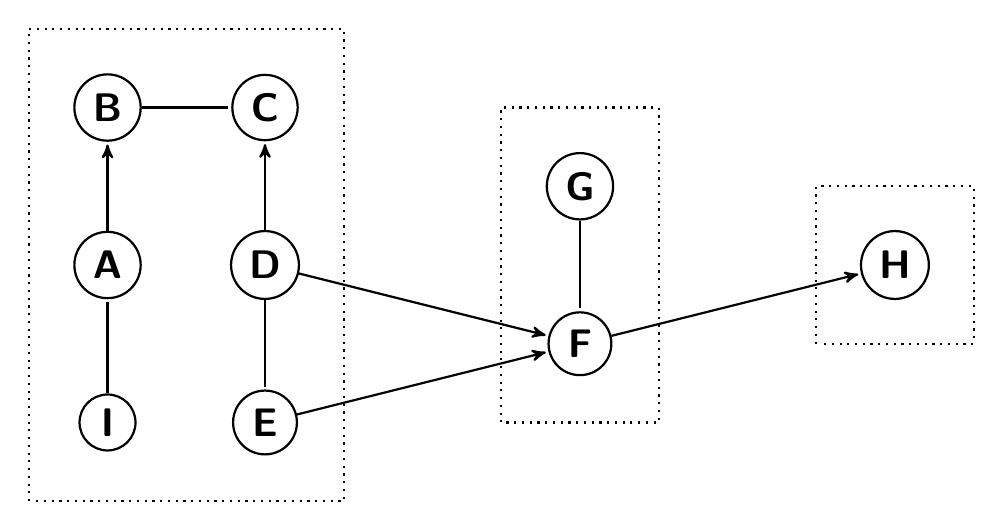
\begin{tikzpicture}[>=stealth',shorten >=1pt,auto,node distance=2.5cm,
		                    thick,main node/.style={circle,draw,font=\sffamily\Large\bfseries}]

			% Rectangles
			\draw[dotted] (-1, -1) -- (-1, 5) -- (3, 5) -- (3, -1) -- (-1, -1);
			\draw[dotted] (5, 0) -- (5, 4) -- (7, 4) -- (7, 0) -- (5, 0);
			\draw[dotted] (9, 1) -- (9, 3) -- (11, 3) -- (11, 1) -- (9, 1);


			% Nodes
			% First block V_1
			\node[main node] (I) at (0, 0) {I};
			\node[main node] (A) at (0, 2) {A};
			\node[main node] (B) at (0, 4) {B};
			\node[main node] (C) at (2, 4) {C};
			\node[main node] (D) at (2, 2) {D};
			\node[main node] (E) at (2, 0) {E};

			% Second block V_2
			\node[main node] (G) at (6, 3) {G};
			\node[main node] (F) at (6, 1) {F};

			% Third block V_3
			\node[main node] (H) at (10, 2) {H};


			% Edges
			\draw (I) -- (A);
			\draw[->] (A) -- (B);
			\draw (B) -- (C);
			\draw[->] (D) -- (C);
			\draw (D) -- (E);

			\draw[->] (D) -- (F);
			\draw[->] (E) -- (F);
			\draw (G) -- (F);

			\draw[->] (F) -- (H);
		\end{tikzpicture}
		
		\caption{$\mc{B}$-consistent labeled block ordering for chain graph \ref{fig:graphForNodeTree}}
		\label{fig:LBOExample}
	\end{figure}
\end{ex}



Ma, Xie and Geng proposed in \cite{CG} algorithm for creating separation tree with labeled block ordering.
Using the main feature of labeled block ordering which is known order of blocks one can construct a DAG of blocks
and then create separation trees from DAG representation of blocks. 

\begin{algorithm}
	\caption{(LCD) Separation Tree Construction with Labeled Block Ordering}

	\textbf{Input:} $\mc{B}$-consistent labeled block ordering $\mc{B} = (V_i^{l_i})_{i = 1}^{k}$ of chain graph $G$ \\
	\textbf{Output:} Separation tree $\mc{T}$ of $G$.

	\begin{algorithmic}[1]
			\State Construct a DAG $D$ with blocks $(V_i)_{i = 1}^{k}$
			\State Construct a junction tree $\mc{T}$ by triangulating $D$
			\State Replace each block $V_i$ in $\mc{T}$ by original vertices it contains
			\State \textbf{return:} $\mc{T}$;
	\end{algorithmic}
	\label{SepLBOAlg}
\end{algorithm}



\begin{ex}
	The following figure [...] presents execution of Algorithm \ref{SepLBOAlg} on labeled block ordering shown in
	figure \ref{fig:LBOExample}. 

	\begin{figure}
		\centering
		\vspace{-10pt}

			
		\begin{tikzpicture}[>=stealth',shorten >=1pt,auto,node distance=2.5cm,
		                    thick,main node/.style={circle,draw,font=\sffamily\Large\bfseries}]
		
			% DAG
			\node (V1) at (0, 0) {$V_1^g$};
			\node (V2) at (2, 2) {$V_2^u$};
			\node (V3) at (4, 0) {$V_3^g$};

			% Boxes
			\draw (-0.35, -0.35) -- (-0.35, 0.35) -- (0.35, 0.35) -- (0.35, -0.35) -- (-0.35, -0.35);
			\draw (1.65, 1.65) -- (1.65, 2.35) -- (2.35, 2.35) -- (2.35, 1.65) -- (1.65, 1.65);
			\draw (3.65, -0.35) -- (3.65, 0.35) -- (4.35, 0.35) -- (4.35, -0.35) -- (3.65, -0.35);

			% DAG edges
			\draw[->] (V1) -- (V2);
			\draw[->] (V2) -- (V3);

			% Subtitle
			\node (subA) at (2, -2) {a)};
		


			% Separation tree
			\node (AB) at (7, 1.5) {A B};
			\node (CDE) at (7, 1) {C D E};
			\node (IGF) at (7, 0.5) {I G F};
			
			\node (GF) at (10, 1) {G F};

			\node (GF) at (12, 1.5) {G F};
			\node (H)  at (12, 1) {H};


			\draw (5.5, 0) -- (7, 2.5) -- (8.5, 0) -- (5.5, 0);
			\draw (8, 1) -- (9.5, 1);
			\draw (9.5, 0.65) -- (9.5, 1.35) -- (10.5, 1.35) -- (10.5, 0.65) -- (9.5, 0.65);

		\end{tikzpicture}
	\end{figure}

\end{ex}


			
			
	\section{Algorithm}
	
		\subsection{Mathematical basis}
			% ----------------------------------------------
%
%	Damian Skrzypiec
% 	August 2017
%	Mathematical basis for LCD algorithm
%
% ----------------------------------------------

There will be mathematical basis for LCD algorithm. In particular theorem $3$ from \cite{CG}.	
	
		\subsection{Skeleton recovery}
			% ----------------------------------------------
%
%	Damian Skrzypiec
% 	August 2017
%	Skeleton recovery algorithm.
%
% ----------------------------------------------


Some info about SKELETON RECOVERY ALG.
[...] The following algorithm was introduced in \cite{CG}, chapter 3.2, algorithm 1.

\begin{algorithm}
	\caption{(LCD) Skeleton Recovery}\label{skeletonRecoveryAlg}
	
	\textbf{Input:} A separation tree $ \mc{T}(G, \mc{C})$; 
					perfect conditional independence knowledge about $\mathbb{P}$.  \\
	\textbf{Output:} The skeleton $G^{'}$ of $G$; a set $\mc{S}$ of c-separators.

	
	\begin{algorithmic}[1]
		\Procedure{RecoverySkeleton($ \mc{T}(G, \mc{C})$)}{}
			\State $\mc{S} = \emptyset$
	
			\ForAll{$\mbox{node} \ C_h \in \mc{T}(G, \mc{C})$} 
				\State	Create complete undirected graph $G_h = (C_h, E_h)$;
				\ForAll{$\mbox{vertex pair} \ \{u, v \} \subset C_h $}
					\If{$\exists S_{uv} \subset C_h \ u \bigCI v \mid S_{uv}$}
						\State Delete edge $(u, v)$ from graph $G_h$;
						\State $\mc{S} := \mc{S} \cup S_{uv}$; \Comment{Add set $S_{uv}$ to separators}
					\EndIf
				\EndFor
			\EndFor			
		
			\State Combine all the graphs $(G_h)_{i \in \{1, \dots, H}$ into undirected graph 
			$G^{'} = (V, \bigcup_{h = 1}^{H} E_h)$;
			
			\ForAll{$ \{u, v \} \in G^{'} \ \mbox{contained in more then 
					one node of} \ \mc{T}(G, \mc{C})$}
				\If{$ \exists C_h \ \{u, v \} \subset C_h \ \mbox{and} \ (u, v) \notin E_h$}
					\State Delete the edge $(u, v)$ from $G^{'}$;
				\EndIf
			\EndFor
			
			\ForAll{$ \{u, v \} \in G^{'} \ \mbox{contained in more then 
					one node of} \ \mc{T}(G, \mc{C})$}
					
				\State $N_{uv} := \{S \subset \mbox{ne}_{G^{'}}(u) \cup \mbox{ne}_{G^{'}}(v) \ | \ 
									S \not\subset C_h \ \mbox{and} \ \{u, v\} \subset C_h  \}$
									
				\If{$u \bigCI v \mid S_{uv} \ \mbox{for some} \ S_{uv} \subset N_{uv}$}
					\State Delete edge $(u, v)$ from graph $G^{'}$;
					\State $\mc{S} := \mc{S} \cup S_{uv}$; \Comment{Add set $S_{uv}$ to separators}
				\EndIf
			\EndFor	
			
			\State \textbf{return:} $G^{'}$, $\mc{S}$.
		\EndProcedure
	\end{algorithmic}
\end{algorithm}


% -----------------------------------
%	Example of application LCD alg.
% -----------------------------------

\begin{ex} \label{skeletonRecoveryEx}
	To illustrate execution of the LCD algorithm let's assume we have data which joint distribution is faithful to
	graph presented in figure \ref{fig:graphForNodeTree} but we do not know it's chain graph representation yet.
	Additionally we have separation tree presented on figure \ref{fig:nodeTree}. 
	Result of first phase of skeleton recovery algorithm is presented on figure \ref{fig:LCDfirstPhaseResult}. 
	For every node tree we have local undirected graph representing local
	(in sense of particular node) independence structure. Phase two of skeleton recovery algorithm join local graphs into
	global undirected graph and removes some of redundant edges. 
	Result of execution second phase is represented on figure
	\ref{fig:LCDsecondPhaseResult}. Result of applying skeleton recovery algorithm is the same as outcome from second
	phase of the algorithm, because there isn't pair of random variable satisfying condition from 20th line of Algorithm 
	\ref{skeletonRecoveryAlg}. Output set of separators in this example is $\mc{S} = \{ \{B\}, \{F \} \}$.

\end{ex}

% -----------------------------------
%	Viz. of I phase of LCD alg.
% -----------------------------------
\begin{figure}
	\centering
	\vspace{-10pt}
	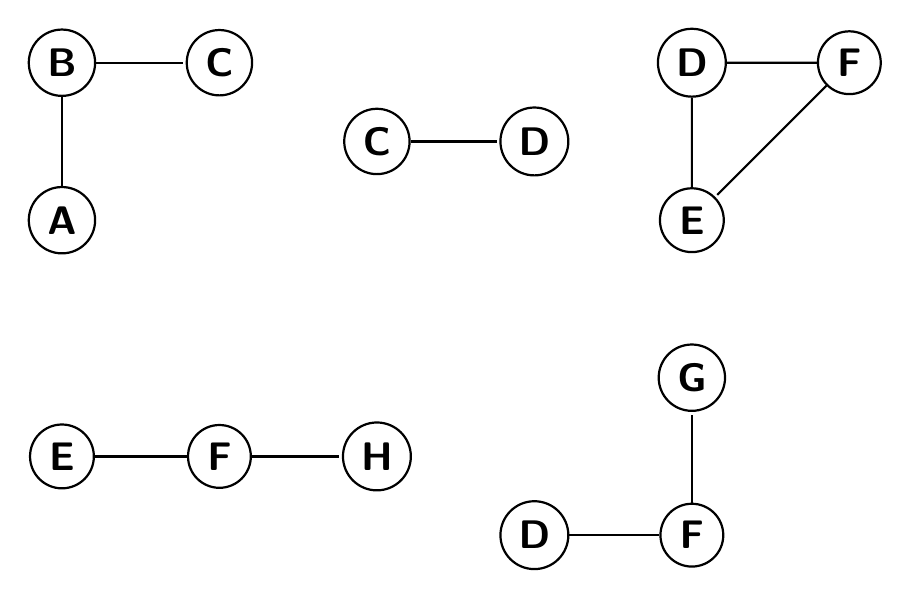
\begin{tikzpicture}[>=stealth',shorten >=1pt,auto,node distance=2.5cm,
	                    thick,main node/.style={circle,draw,font=\sffamily\Large\bfseries}]
		% Nodes
		  %Row1
		  \node (A1) at (0, 2) [main node] {A};
		  \node (B1) at (0, 4) [main node] {B};
		  \node (C1) at (2, 4) [main node] {C};
		  
		  \node (C2) at (4, 3) [main node] {C};
		  \node (D2) at (6, 3) [main node] {D};
		  
		  \node (D3) at (8, 4) [main node] {D};
		  \node (E3) at (8, 2) [main node] {E};
		  \node (F3) at (10, 4) [main node] {F};
		  
		  % Row2
		  \node(E4) at (0, -1) [main node] {E};
		  \node(F4) at (2, -1) [main node] {F};
		  \node(H4) at (4, -1) [main node] {H};
		  
		  \node(D5) at (6, -2) [main node] {D};
		  \node(F5) at (8, -2) [main node] {F};
		  \node(G5) at (8, 0) [main node] {G};			
		
		% Edges
		  \draw (A1) -- (B1) -- (C1);
		  \draw (C2) -- (D2);
		  \draw (E3) -- (D3) -- (F3) -- (E3);			  
		  
		  \draw (E4) -- (F4) -- (H4);
		  \draw (D5) -- (F5) -- (G5);
		  
		\end{tikzpicture}
		
	\caption{Result of first phase of LCD algorithm}			
	\label{fig:LCDfirstPhaseResult} 
\end{figure}




% -----------------------------------
%	Viz. of II phase of LCD Alg
% -----------------------------------
\begin{figure}
		\centering
		\vspace{-10pt}
		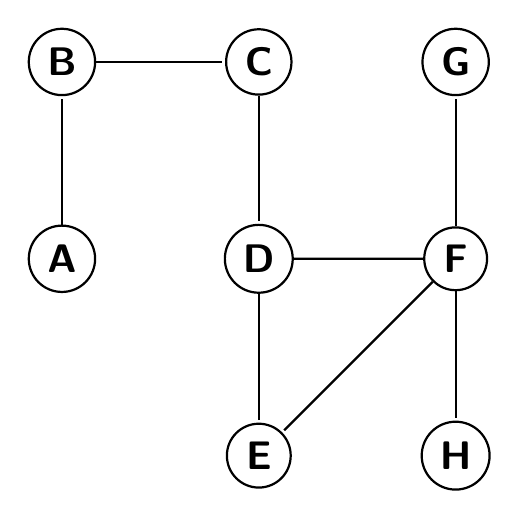
\begin{tikzpicture}[>=stealth',shorten >=1pt,auto,node distance=2.5cm,
		                    thick,main node/.style={circle,draw,font=\sffamily\Large\bfseries}]
			% Nodes
			  \node[main node] (A) {A};
			  \node[main node] (B) [above of = A] {B};
			  \node[main node] (C) [right of = B] {C};
			  \node[main node] (D) [below of = C] {D};
			  \node[main node] (E) [below of = D] {E};
			  \node[main node] (F) [right of = D] {F};
			  \node[main node] (G) [above of = F] {G};
			  \node[main node] (H) [below of = F] {H};			
			
			% Edges
			  \draw (A) -- (B);
			  \draw (B) -- (C);
			  \draw (C) -- (D);
			  \draw (D) -- (F) -- (E);
			  \draw	(D) -- (E);
			  \draw (F) -- (G);
			  \draw (F) -- (H);
			\end{tikzpicture}
			
		\caption{Result of second phase of LCD algorithm}			
		\label{fig:LCDsecondPhaseResult} 
	\end{figure}	
	
		\subsection{Complexes recovery}
			% ----------------------------------------------
%
%	Damian Skrzypiec
% 	August 2017
%	Complex recovery algorithm (LCD)
%
% ----------------------------------------------

Some words. The following algorithm was introduced in \cite{CG}, chapter 3.3, algorithm 2.

\begin{algorithm}
	\caption{(LCD) Complex Recovery}\label{complexRecoveryAlg}
	
	\textbf{Input:} Perfect conditional independence knowledge about $\mathbb{P}$; the skeleton $G^{'}$ and the set 
					$\mc{S}$ of c-separators obtained in algorithm \ref{skeletonRecoveryAlg}.  \\
	\textbf{Output:} The pattern $G^{*}$ of graph $G$.

	
	\begin{algorithmic}[1]
		\Procedure{ComplexRecovery($ \mc{T}(G, \mc{C})$)}{}
			\State Initialize $G^{*} = G^{'}$ 
	
			\ForAll{$\mbox{ordered pair} \ [u, v] \ : S_{uv} \in \mc{S}$} 
				\ForAll{$ u - w \ \mbox{in} \ G^{*}$}
					\If{$ u \not \bigCI v \mid S_{uv} \cup \{ w \} $}
						\State Orient $u - w$ as $u \rightarrow w$ in $G^{*}$;
					\EndIf
				\EndFor
			\EndFor			
			
			\State \textbf{return:} Pattern of $G^{*}$.
		\EndProcedure
	\end{algorithmic}
\end{algorithm}


\begin{ex}
	In this example we present performance of complex recovery algorithm for outcomes from skeleton recovery
	algorithm presented in Example \ref{skeletonRecoveryEx}. If we consider pair $[D, A]$ in outer loop in
	the algorithm we find that $S_{DA} = \{ B \}$ and $D \not \bigCI A \mid \{ B \} \cup \{ C \}$, therefore 
	we orient edge $D \rightarrow C$. Similar we orient edge $A \rightarrow B$, because for pair $[A, D]$ in
	the outer loop we have $S_{AD} = \{ B \}$ and $A \not \bigCI D \mid \{ B \} $. Conditional independence 
	in this case is not satisfied because condition $\cSep{A}{D}{B}{G}$ does not hold and we have assumption
	of faithfulness. For $[D, G]$ in outer loop we have $S_{DG} = \{ F\}$ and 
	$D \not \bigCI G \mid S_{DG} \cup \{ F \}$, hence we orient edge $D \rightarrow F$. Orientation of edge 
	$E \rightarrow F$ is obtained by consideration $[E, H]$ in outer loop and $w = F$. Result of complex
	recovery algorithm is presented in figure \ref{fig:ComplexREcoveryResult}. The edge $[F, H]$ was not oriented
	by the algorithm because condition $F \not\bigCI H \mid F$ is not satisfied. As we mentioned before 
	LCD algorithm creates representative of Markov equivalence class of given chain graph. 
	Chain graphs presented in figure \ref{fig:ComplexREcoveryResult} and \ref{fig:graphForNodeTree} are in the
	same Markov equivalence class.  
\end{ex}


% For Test -- -- --  
% -----------------------------------
%	Viz. of complex recovery alg
% -----------------------------------
\begin{figure}
		\centering
		\vspace{-10pt}
		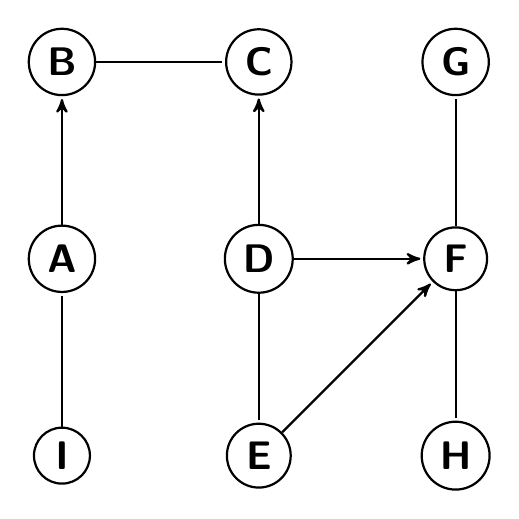
\begin{tikzpicture}[>=stealth',shorten >=1pt,auto,node distance=2.5cm,
		                    thick,main node/.style={circle,draw,font=\sffamily\Large\bfseries}]
			% Nodes
			  \node[main node] (A) {A};
			  \node[main node] (B) [above of = A] {B};
			  \node[main node] (C) [right of = B] {C};
			  \node[main node] (D) [below of = C] {D};
			  \node[main node] (E) [below of = D] {E};
			  \node[main node] (F) [right of = D] {F};
			  \node[main node] (G) [above of = F] {G};
			  \node[main node] (H) [below of = F] {H};			
			  \node[main node] (I) [below of = A] {I};			
			
			% Edges
			  \draw     (I) -- (A);
			  \draw[->] (A) -- (B);
			  \draw     (B) -- (C);
			  \draw[->] (D) -- (C);
			  \draw[->] (D) -- (F);
			  \draw	    (D) -- (E);
			  \draw[->] (E) -- (F);
			  \draw     (F) -- (G);
			  \draw     (F) -- (H);
			\end{tikzpicture}
			
		\caption{Result of Complex Recovery Algorithm}			
		\label{fig:ComplexREcoveryResult} 
\end{figure}

	
		\subsection{Algorithm complexity}
			% ----------------------------------------------
%
%	Damian Skrzypiec
% 	August 2017
%	Algorithm Comp. Complexity of LCD alg.
%
% ----------------------------------------------



The skeleton and complex recovery phases are independent in sense of computational complexity, hence we can
find upper bounds for those two phases separately. 
Let suppose that we have unknown chain graph 
$G = (V, E)$ with $|V| = n$ and $|E| = m$. Let further suppose that the input separation tree $\mc{T}$ contains 
tree nodes
$H = \{ C_1, C_2, \dots, C_k \}$. To denote number of elements of separation tree node $C_i$ we use $c_i$ and by
$m$ we denote count of the biggest node in separation tree, that is $m = \max \{ c_i \ | \ i \in \{1, 2, \dots, k \} \}$.

The most computational expensive step in the skeleton recovery algorithm is loop in line 5 and verifying 
condition in line 6 of Algorithm \ref{skeletonRecoveryAlg}. For given node in the separation tree $C_i$ looping over
all pairs $\{u, v\} \subset C_i$ is of complexity $\frac{1}{2} c_i \cdot (c_i + 1)$ which is $\mc{O}(c_i^2)$. For given node in the separation
tree and given pair of vertex $\{u, v\}$ verifying condition in line 6 of Algorithm \ref{skeletonRecoveryAlg} is of
cost $2^{c_i}$ because it requires to look over all subsets of $C_i$. Second and third steps of the skeleton
recovery algorithm are less computational complex then the first step. Therefore complexity of the whole algorithm 
is determined by complexity of the first step which can be estimated as follow


\begin{equation}
\begin{split}
	T(\mc{T}) & = \mc{O} \left( \sum_{C_i \in H} \frac{1}{2} c_i (c_i + 1) 2^{c_i} \right)  \le  \\
	&  \le \mc{O} \left( \sum_{C_i \in H} \frac{1}{2}m(m+1)2^{m} \right) =  \\
	& = \mc{O} \left( km^2 2^m \right)
\end{split}
\end{equation}







			
			
\chapter{ASP Algorithm}


\begin{thebibliography}{99}
	\addcontentsline{toc}{chapter}{Bibliography}
	\bibitem{CGMP} M. Frydenberg, \textit{The Chain Graph Markov Property}, Scandinavian Journal of Statistics 17 (1990) 333-353	
	
	\bibitem{UGM} R. D. Nowak and D. Vats, \textit{A Junction Tree Framework for Undirected Graphical Model Selection}, Journal of Machine Learning Research 15 (2014) 147-191
	
	\bibitem{CG} Z. Ma, X. Xie and Z. Geng, \textit{Structural Learning Of Chain Graphs via Decomposition}, Journal of Machine Learning Research 9 (2008) 2847-2880

	\bibitem{OCG} M. Studeny and R.R. Bouckaert, \textit{On chain graph models for description of conditional independence structures}, Annals Of Statistics 26 (1998) 1434-1495
	
\end{thebibliography}

\end{document}


%%% Local Variables:
%%% mode: latex
%%% TeX-master: t
%%% coding: latin-2
%%% End:
